
\section{Einführung in die Microfrontend Architektur}

Diese Arbeit vergleicht Architektur-Alternativen für die Verteilung des Frontends auf die Services. Der Text wird die Architektur beschreiben, die Chancen und Risiken anhand eines Kriterienkataloges untersuchen. Diese Kriterien werden verwendet um die ausprogrammierten Alternativen zu vergleichen. Das letzte Kapitel wird die gewonnen Fakten über die Architekturalternativen vergleichen und bewerten.

Der Begriff \enquote{Microservices} \marg{Microservices} ist in einem Software-Architektur-Workshop in Mai 2011 aufgekommen \cite{ieeeJournal2018}. Microservices werden als \enquote{lose gekoppelte \ac{SOA} mit einem begrenzten Kontext}\cite{cockcroft2016} beschrieben. Vielfach wird diese neuartige Architektur bei Webservices mit aktuellen Technologien wie \ac{JSON} und \ac{REST} verbunden. 

Die Applikationsschicht wurde in verschiedene Services aufgeteilt, aber die Präsentationsschicht ist zurzeit eine grosse Website, die alle Services überspannt. Das Frontend übernimmt die Koordinierung, damit die Services in der richtigen Reihenfolge aufgerufen werden. Beispielsweise ist im Bild \ref{fig:requirements:introduction:traditional} der Login-Service ersichtlich, der vor den anderen Services aufgerufen werden muss um den Nutzer zu authentisieren.

Dies hat den Nachteil, dass in der Präsentationsschicht Code für verschiedene Services miteinander verhängt ist. Dadurch verlieren wir den grossen Vorteil von Microservices, ihre Unabhängigkeit voneinander. Es existieren keine logischen Barrikaden zwischen den Frontends. Aus diesem Grund kann der gesammte Code auf jede Service API zugreifen. Es existieren keine klar definierten Zuständigkeiten. Ausserdem muss jeder Entwickler im Frontend die gleichen Abhängigkeiten benutzen. Als Beispiel muss der gesammte Frontend-Code auf Angular\footnote{\url{https://angular.io}} aufgesetzt werden.

\begin{figure}
    \centering
    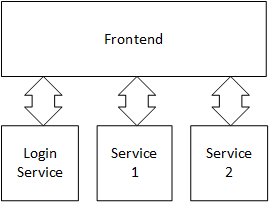
\includegraphics{./sections/requirements/assets/TraditionalArchitecture}
    \caption{A traditionelle Service Architektur}
    \label{fig:requirements:introduction:traditional}
\end{figure}

Das \marg{Microfrontends} \textit{Microfrontend} Konzept nimmt die Vorteile, die in der \textit{Applikationsschicht} mit dem \textit{Microservices} Konzept gewonnen wurden, in die Präsentation-Schicht. Wir unterteilen das \ac{UI} in selbst-verwaltende Subsysteme, welche per Definition nur  zu ihrem Microservice kommunizieren. Die Kombination von Microservice und Microfrontend sind selbst-verwaltend und ein geschlossenes System.

Unter \ref{fig:requirements:introduction:microfrontend} ist der Aufbau von Microfrontends ersichtlich. Der Service liefert sein eigenes UI, das als Teil der übergeordneten Seite einfach eingefügt wird. Somit ist jeder Service im Frontend unabhängig von der verwendeten Technologie bei den anderen Services. Die Microfrontends haben auch die Aufgabe mit dem Service zu kommunizieren und teilen die Daten über ein Message-System anderen Microfrontends im Browser mit. Die Funktionsweise eines solchen Messaging-Systems ist ausserhalb des Umfangs dieser Arbeit und wurde in anderen Arbeiten\footnote{https://medium.com/@tomsoderlund/micro-frontends-a-microservice-approach-to-front-end-web-development-f325ebdadc16\#3b29} untersucht.

\begin{figure}
    \centering
    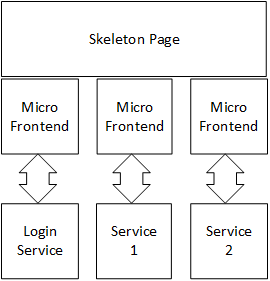
\includegraphics{./sections/requirements/assets/MicroFrontendArchitecture}
    \caption{Mikrofrontend Architektur}
    \label{fig:requirements:introduction:microfrontend}
\end{figure}

Microfrontends \marg{Vorteile} haben eine breite Palette von Vorteilen. Von einer technischen Perspektive, der Code ist modularisierter, Komponenten sind austauschbar in Produktion und sie unterteilen die Applikation in kleinere Sicherheitsbereiche. Die Microfrontends könnnen die Präsenz von der Skeleton Page erwarten. Beispielsweise können die Microfrontends Nachrichten über einen gemeinsamen Message-Bus\cite{Curry2005} austauschen.\cite{Söderlund2017} 

Das Pattern könnte den Entwicklungsprozess von Webservices grundlegend verändern. Jedes Microfrontend kann individuell programmiert werden, auf die Produktionsumgebung geladen werden und instand gehalten werden. Die Aufsicht kann durch ein kleines und unabhängiges Team gewahrt werden. Die Teams müssen sich nicht untereinander absprechen beim Aktualisieren der Software, denn der Frontend-Code ist unabhängig voneinander.

Auf der anderen Seite, \marg{Risiken} ist die Implementierung der Microservice- und Microfrontend-Patterns aufwendig und verzögert die Entwicklung von neuen Funktionen. Ausserdem kann das Einsetzen von verschiedenen UI-Hilfsbibliotheken viele Ressourcen im Browser brauchen, zum Beispiel haben viele aufwendige Webservices einen hohen Hauptspeicherverbrauch auf der Nutzermaschine.

Die Trennung der Code-Abhängigkeiten kann zur Verletzung des \textit{dont repeat yourself} Prinzipes\cite{Hunt2008} führen. Die Javascript-Bibliotheken, auf denen die Microfrontends basieren, muss mehrmals zum Code compiliert werden.
\newpage